\subsection{\texorpdfstring{$y''-xy = 0$}{y''-xy = 0}}
Die Koeffizienten der uns bereits bekannten Airy-Differentialgleichung k"onne 
durch einfaches Einsetzen in die Formel (\ref{eq:wellen:allgemeineak}) 
berechnet werden.

\begin{equation*}
	\begin{split}
		a_k &= -\frac{1}{k(k-1)} ((-1) a_{k-2-1} + 
		0 a_{k-2-0})
		\\
		&= \frac{1}{k(k-1)} a_{k-3}, \qquad a_{k < 0} = 0,
	\end{split}
\end{equation*}
was sich mit den bereits bekannten L"osung deckt.

Auch die genannten Konsequenzen werden in der Abbildung 
\ref{fig:wellen:airy-dgl} deutlich aufgezeigt.

\begin{figure}
	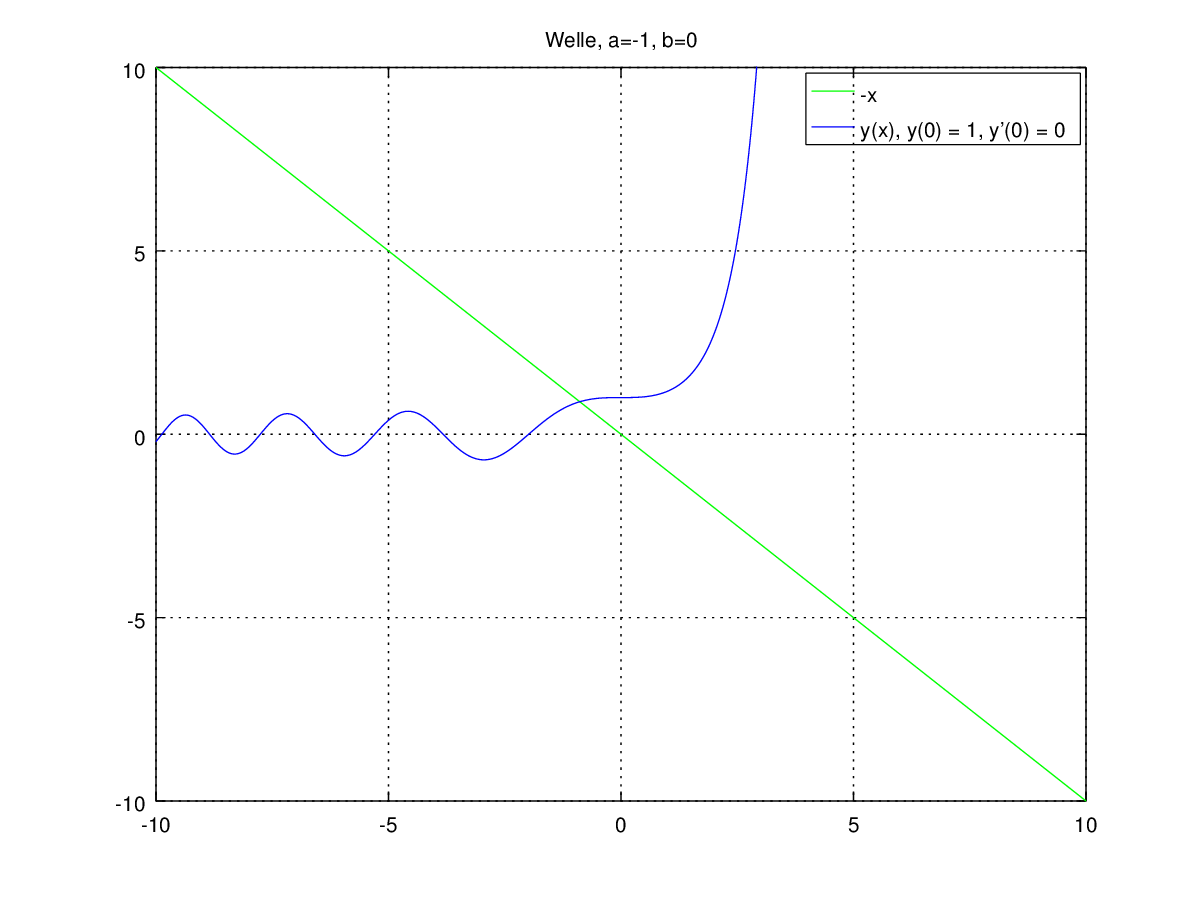
\includegraphics[scale=0.65]{./wellen/images/allgemein/n1.png}
	\caption{L"osung Airy-Differentialgleichung}
	\label{fig:wellen:airy-dgl}
\end{figure}